\documentclass[mathserif,11pt]{beamer}

\usepackage{url,verbatim,natbib}
\usepackage[english]{babel}
\usepackage{amsmath, mathabx}
\usepackage{dsfont, ulem}
\usepackage{tikz}
\usepackage{xparse}
\newtheorem{proposition}[theorem]{Proposition}

\usepackage[headheight=22pt]{beamerthemeboxes}
\usepackage{graphicx}
\beamertemplatenavigationsymbolsempty 
\setbeamercovered{transparent}
\usepackage{centernot}

\setbeamertemplate{itemize item}{$\bullet$} 
\setbeamercolor{title}{fg=uio}
\setbeamertemplate{sections/subsections in toc}[ball unnumbered]
\setbeamercolor{section in toc}{fg=uio,bg=white}
\setbeamercolor{subsection in toc}{fg=uio,bg=white}
\setbeamercolor{result}{fg=black, bg=yellow}
\newcommand{\dotsim}{\stackrel{\cdot}{\sim}}
\newcommand{\interi}{{\rm Z}\negthinspace\negthinspace {\rm Z}}
\newcommand{\reali}{{\rm I}\negthinspace {\rm R}}
\newcommand{\naturali}{{\rm I}\negthinspace {\rm N}}
\newcommand{\sign}{\mathop{\rm sgn}\nolimits}
\newcommand{\sgn}{\mathop{\mathrm{sgn}}}
\definecolor{redve}{rgb}{0.604,0.008,0.00}
\definecolor{lmu}{rgb}{0.188,0.522,0.306}
\definecolor{uio}{rgb}{0.847,0.118,0.02}

\def\R{{\rm I\!R}}
\def\P{{\rm Pr}}
\def\Real{{\rm I\!R}}
\def\T{{\footnotesize {^{_{\sf T}}}}}
\def\tr{{\rm tr}}
\def\diag{{\rm diag}}

\NewDocumentCommand\DownArrow{O{2.0ex} O{black}}{%
   \mathrel{\tikz[baseline] \draw [<-, line width=0.5pt, #2] (0,0) -- ++(0,#1);}
}

\useframetitletemplate{% 
\begin{centering} 
\begin{small} \structure{\textcolor{uio} \insertframetitle {\insertframesubtitle}}
\end{small}

\end{centering} 
}

\addheadboxtemplate{\color[rgb]{1,1,1}}{\color{uio} \underline{{\hspace{5pt}\includegraphics[scale=0.06]{../../../../support/uio_logo_eng} \hspace{0.265\paperwidth}\color{black} \tiny  STK-IN4300 - Statistical Learning Methods in Data Science} \hspace{5pt}}}

%\bfseries{\insertsection}

\addfootboxtemplate{\color[rgb]{1,1,1}}{\color{black} \tiny \quad  
STK-IN4300: lecture 8
  \hfill \tiny \insertframenumber / \inserttotalframenumber \hspace{5pt}}

  
\title{STK-IN4300 \\ Statistical Learning Methods in Data Science}
\author{Riccardo De Bin} 
\institute{debin@math.uio.no} 
\date{}


\begin{document}
\setbeamercolor{bgr}{fg=black,bg=uio}

{
\setbeamertemplate{headline}{}
\frame{
\vspace{-2cm}
\begin{beamercolorbox}[sep=-2.2em,wd=5cm,colsep=0.5pt,ht=4.25ex,dp=3ex,left]{postit}
\includegraphics[scale=0.06]{../../../../support/uio_logo_eng}
\end{beamercolorbox}
\vspace{0.365cm}
\noindent\makebox[\linewidth]{\color{uio} \rule{\paperwidth}{0.4pt}}
\vspace{2.5cm}
\titlepage
}
}

\frame{\frametitle{Outline of the lecture}
\tableofcontents
}


\section{Generalized Additive Models}

\subsection{Definition}

\frame{\frametitle{Generalized Additive Models: }
\framesubtitle{introduction}
From the previous lecture:
\begin{itemize}
\item \textcolor{uio}{linear regression model} are easy and effective models;
\item often the effect of a predictor on the response is \textcolor{uio}{not linear};
\item[] \centering $\downarrow$
\item[] \textcolor{uio}{local polynomials} and \textcolor{uio}{splines}.
\end{itemize}

\vspace{12pt}

{\bf \uline{Generalized Additive Models}}:
\begin{itemize}
\item flexible statistical methods to identify and characterize \textcolor{uio}{nonlinear regression} effects;
\item lerger class than the generalized linear models.
\end{itemize}
}


\frame{\frametitle{Generalized Additive Models: }
\framesubtitle{additive models}
Consider the usual framework:
\begin{itemize}
 \item $X_1, \dots, X_p$ are the predictors;
 \item $Y$ is the response variable;
 \item $f_1(\cdot), \dots, f_p(\cdot)$ are \textcolor{uio}{unspecified smooth functions}.
 \item[]
\end{itemize} 
Then, an {\bf \uline{additive model}} has the form
$$
E[Y|X_1,\dots,X_p] = \alpha + f_1(X_1) + \dots + f_p(X_p).
$$
}


\frame{\frametitle{Generalized Additive Models: }
\framesubtitle{more generally}
As linear models are extended to generalized linear models, we can generalized the additive models to the \textcolor{uio}{generalized additive models},
$$
g(\mu(X_, \dots, X_p)) = \alpha + f_1(X_1) + \dots + f_p(X_p),
$$
where:
\begin{itemize}
\item $\mu(X_1, \dots, X_p) = E[Y|X_1,\dots,X_p]$ is the \textcolor{uio}{link function};
\item $g(\mu(X_1, \dots, X_p))$ is the link function;
\item classical examples:
\begin{itemize}
\item $g(\mu)=\mu$ $\leftrightarrow$ \textcolor{uio}{identity link} $\rightarrow$ Gaussian models;
\item $g(\mu)=\log(\mu/(1-\mu))$ $\leftrightarrow$ \textcolor{uio}{logit link} $\rightarrow$ Binomial models;
\item $g(\mu)=\Phi^{-1}(\mu)$ $\leftrightarrow$ \textcolor{uio}{probit link} $\rightarrow$ Binomial models;
\item $g(\mu)=\log(\mu)$ $\leftrightarrow$ \textcolor{uio}{logarithmic link} $\rightarrow$ Poisson models;
\item \dots
\end{itemize}
\end{itemize}
}


\frame{\frametitle{Generalized Additive Models: }
\framesubtitle{semiparametric models}
Generalized additive models are very \textcolor{uio}{flexible}:
\begin{itemize}
\item \textcolor{uio}{not all} functions $f_j(\cdot)$ must be nonlinear;
$$
g(\mu) = X^T\beta + f(Z)
$$
in which case we talk about {\bf \uline{semiparametric models}}.
\item nonlinear effect can be \textcolor{uio}{combined with qualitative} inputs,
$$
g(\mu) = f(X) + g_k(Z) = f(X) + g(V,Z)
$$
where $k$ indexes the \textcolor{uio}{level} of a qualitative variable $V$.
\end{itemize}
}


\subsection{Fitting algorithm}
\frame{\frametitle{Fitting algorithm: }
\framesubtitle{difference with splines}
When implementing \textcolor{uio}{splines}:
\begin{itemize}
\item each function is modelled by a \textcolor{uio}{basis expansion};
\item the resulting model can be \textcolor{uio}{fitted} with \textcolor{uio}{least squares}.
\item[]
\end{itemize}
Here the approach is \textcolor{uio}{different}:
\begin{itemize}
\item \textcolor{uio}{each function} is modelled with a \textcolor{uio}{smoother} (smoothing splines, kernel smoothers, \dots)
\item all $p$ functions are \textcolor{uio}{simultaneously} fitted via an algorithm.
\end{itemize}
}


\frame{\frametitle{Fitting algorithm: }
\framesubtitle{ingredients}
Consider an additive model
$$
Y = \alpha + \sum_{j=1}^p f_j(X_j) + \epsilon.
$$
We can define a \textcolor{uio}{loss function},
$$
\sum_{i=1}^N \left(y_i - \alpha  - \sum_{j=1}^p f_j(x_{ij})\right)^2 + \sum_{j=1}^p\lambda_j\int\{f_j''(t_j)\}^2 dt_j
$$
\begin{itemize}
\item $\lambda_j$ are \textcolor{uio}{tuning} parameters;
\item the \textcolor{uio}{minimizer} is an additive \textcolor{uio}{cubic spline} model,
\begin{itemize}
\item each $f_j(X_j)$ is a cubic spline with knots at the (unique) $x_{ij}$'s.
\end{itemize}
\end{itemize}
}


\frame{\frametitle{Fitting algorithm: }
\framesubtitle{constrains}
The parameter $\alpha$ is in general \textcolor{uio}{not identifiable}:
\begin{itemize}
\item same result if adding a \textcolor{uio}{constant} to each $f_j(X_j)$ and subtracting it from $\alpha$;
\item by convention, \textcolor{uio}{$\sum_{j=1}^p f_j(X_j) = 0$}:
\begin{itemize}
\item the functions \textcolor{uio}{average 0} over the data;
\item $\alpha$ is therefore \textcolor{uio}{identifiable};
\item in particular, $\hat{\alpha} = \bar{y}$.
\item[]
\end{itemize}
\end{itemize}
If this is true and the matrix of inputs $X$ has full rank:
\begin{itemize}
\item the loss function is \textcolor{uio}{convex};
\item the \textcolor{uio}{minimizer is unique}.
\end{itemize}
}


\frame{\frametitle{Fitting algorithm: }
\framesubtitle{backfitting algorithm}
The {\bf \uline{backfitting algorithm}}:
\begin{enumerate}
\item Initialization: $\hat{\alpha}=N^{-1}\sum_{i=1}^N y_i$ and $\hat{f}_j \equiv 0$ $\forall j$
\item In cycle, $j = 1, \dots, p, 1, \dots, p, \dots$
$$
\hat{f}_j \leftarrow \mathcal{S}_j\left[\{y_i - \alpha  - \sum_{k\neq j} \hat{f}_k(x_{ik})\}_1^N\right]
$$
$$
\hat{f}_j \leftarrow \hat{f}_j - \frac{1}{N}\sum_{i=1}^N \hat{f}_j(x_{ij})\}
$$
until $\hat{f}_j$ change less than a \textcolor{uio}{pre-specified threshold}.
\end{enumerate}
$\mathcal{S}_j$ is \textcolor{uio}{usually} a cubic smoothing spline, but other smoothing operators can be used.
}


\frame{\frametitle{Fitting algorithm: }
\framesubtitle{remarks}
Note:
\begin{itemize}
\item the smoother $\mathcal{S}$ can be (when applied only at the training points) represented by the $N\times N$ \textcolor{uio}{smoothing matrix $S$},
\begin{itemize}
\item the degrees of freedom for the $j$-th terms are \textcolor{uio}{trace$(S)$};
\end{itemize}
\item for the generalized additive model, the loss function is the \textcolor{uio}{penalized log-likelihood};
\item the backfitting algorithm fits \textcolor{uio}{all predictors},
\begin{itemize}
\item not feasible when $p >> N$.
\end{itemize}
\end{itemize}
}
 


\section{Tree-based Methods}

\subsection{Background}

\frame{\frametitle{Tree-based Methods: }
\framesubtitle{introduction}
Consider a \textcolor{uio}{regression} problem, $Y$ the response, $X$ the input matrix.

\vspace{12pt}

A tree is a \textcolor{uio}{recursive binary partition} of the feature space:
\begin{itemize}
\item each time a region is \textcolor{uio}{divide} in two or more regions;
\begin{itemize}
\item until a \textcolor{uio}{stopping criterion} applies;
\end{itemize}
\item at the end, the \textcolor{uio}{input space is split} in $M$ regions \textcolor{uio}{$R_{m}$};
\item a \textcolor{uio}{constant $c_{m}$} is fitted to each $R_{m}$.
\end{itemize}
The \textcolor{uio}{final prediction} is
$$
\hat {f}(X) = \sum_{m=1}^M \hat{c}_{m}\mathds{1}(X \in R_{m}),
$$
where $\hat{c}_{m}$ is an \textcolor{uio}{estimate} for the region $R_m$ (e.g., $\text{ave}(y_i|x_{i} \in R_{m})$).
}


\frame{\frametitle{Tree-based Methods: }
\framesubtitle{introduction}
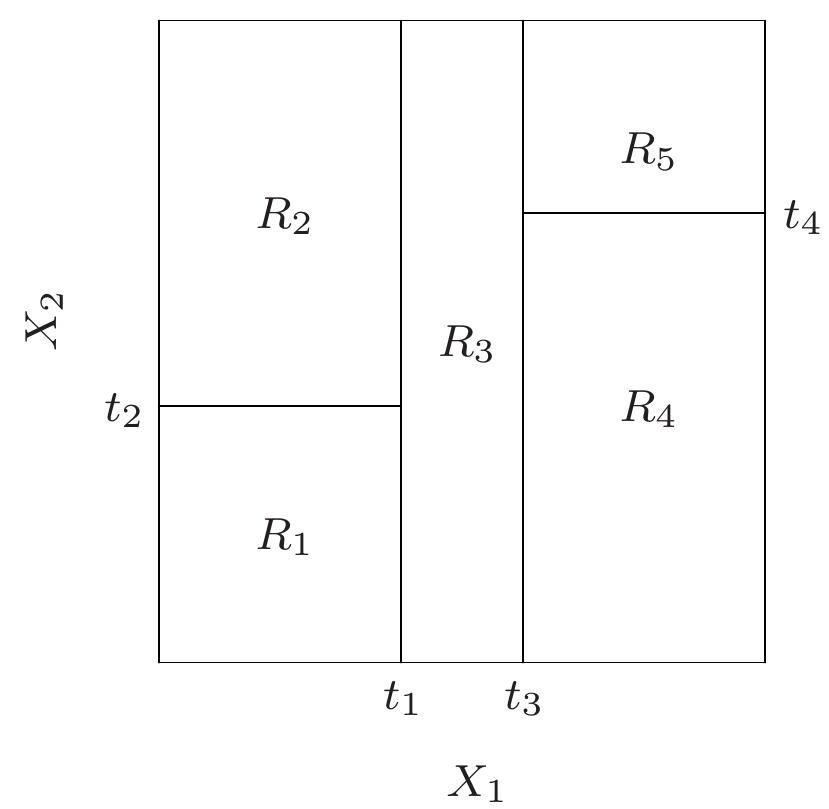
\includegraphics[width=0.49\textwidth]{fig9_21}
\hspace{2pt}
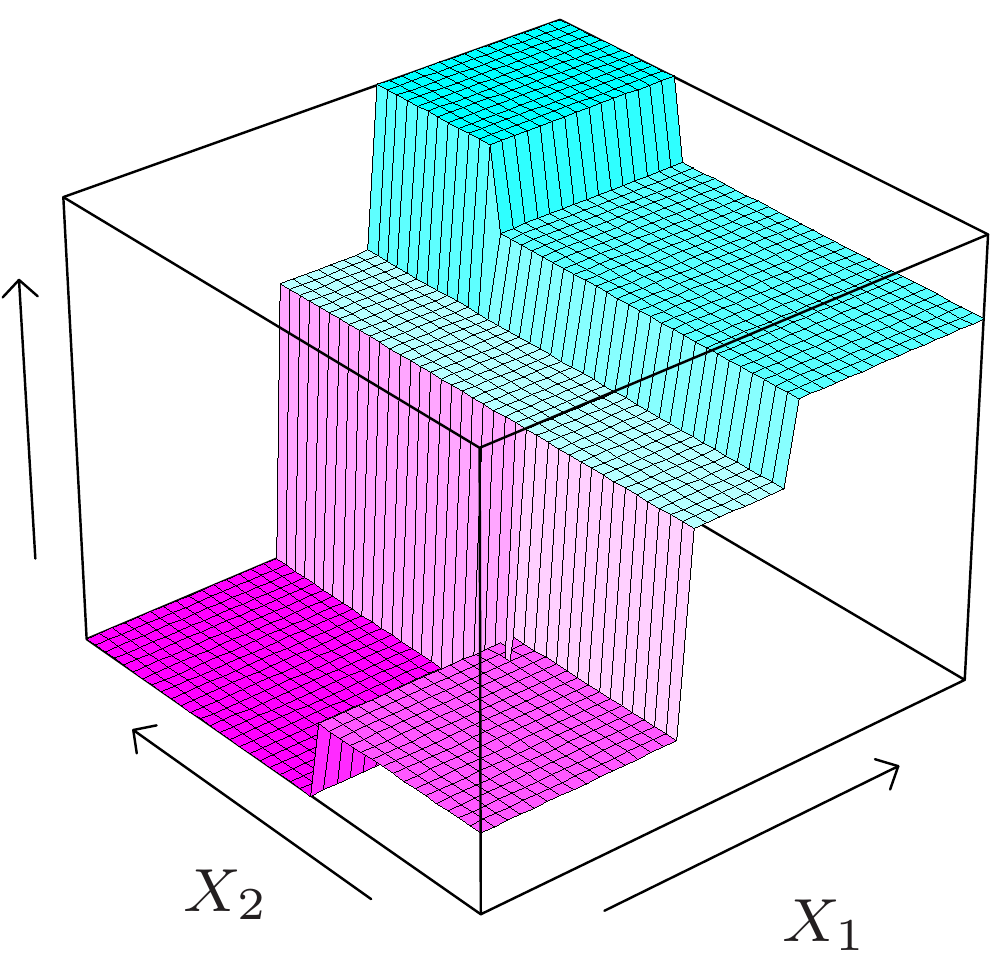
\includegraphics[width=0.49\textwidth]{fig9_23}
}


\frame{\frametitle{Tree-based Methods: }
\framesubtitle{introduction}
Note:
\begin{itemize}
\item the split can be represented as a \textcolor{uio}{junction} of a \textcolor{uio}{tree};
\item this representation works for \textcolor{uio}{$p>2$};
\item each observation is \textcolor{uio}{assigned to a branch} at each junction;
\item[]
\item the model is \textcolor{uio}{easy to interpret}.
\end{itemize}
}


\frame{\frametitle{Tree-based Methods: }
\framesubtitle{introduction}
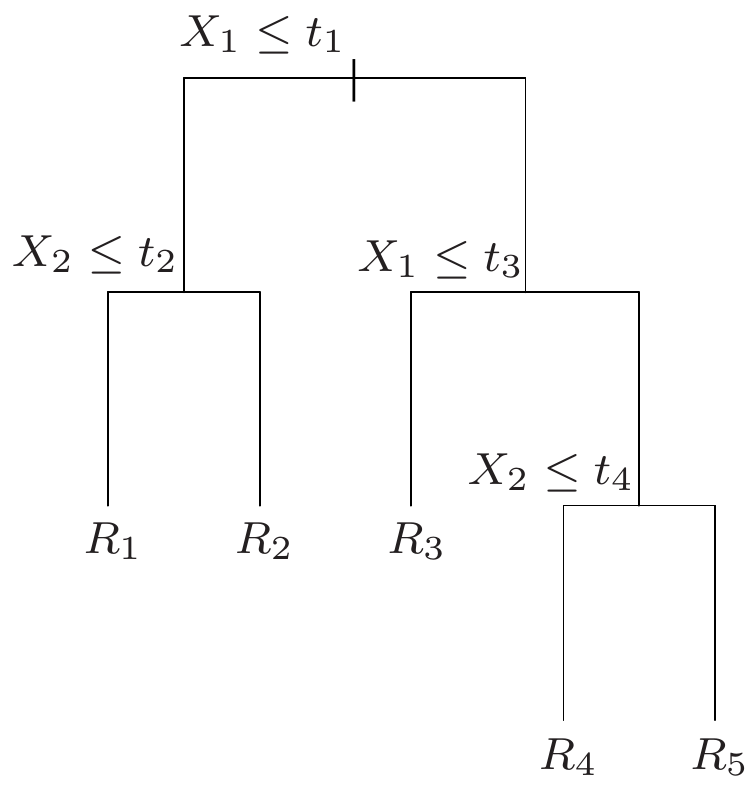
\includegraphics[width=0.49\textwidth]{fig9_22}
\hspace{2pt}
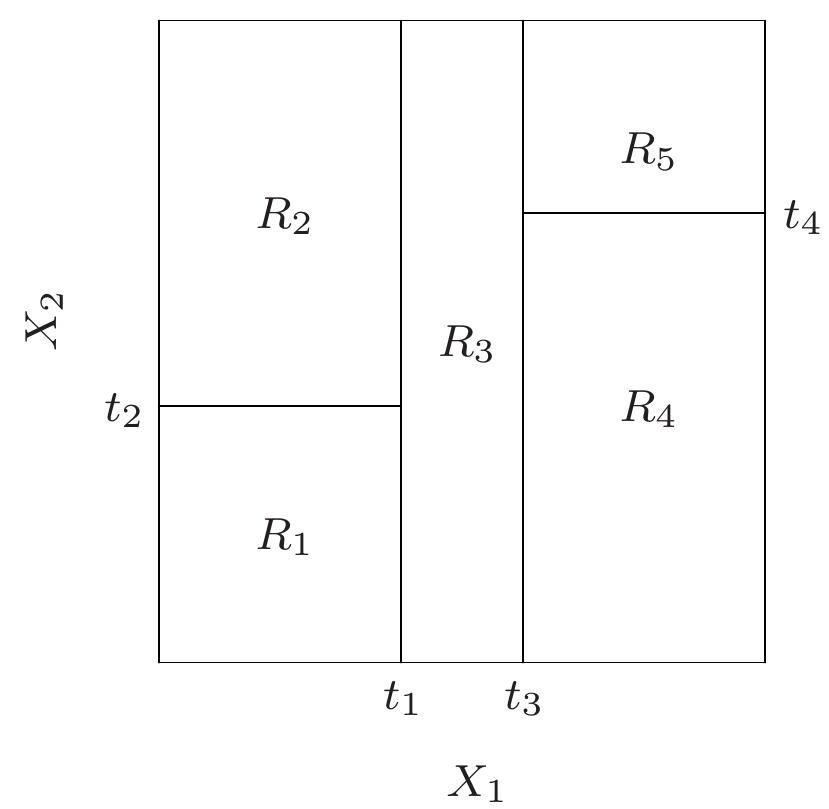
\includegraphics[width=0.49\textwidth]{fig9_21}
}


\subsection{How to grow a regression tree}

\frame{\frametitle{How to grow a regression tree: }
\framesubtitle{split}
How to \textcolor{uio}{grow} a regression tree:
\begin{itemize}
\item we need to automatically decide the \textcolor{uio}{splitting variables} \dots
\item \dots and the \textcolor{uio}{splitting points};
\item we need to decide the \textcolor{uio}{shape} (topology) of the tree.
\item[]
\end{itemize}

Using a \textcolor{uio}{sum of squares} criterion, $\sum_{i=1}^N (y_i - f(x_i))^2$,
\begin{itemize}
\item the best $\hat{c}_m = \text{ave}(y_i|x_{i} \in R_{m})$;
\item finding the \textcolor{uio}{best partition} in terms of minimum sum of squares is generally \textcolor{uio}{computationally infeasible}
\item[] \centering $\downarrow$
\item[] go \textcolor{uio}{greedy}
\end{itemize}
}


\frame{\frametitle{How to grow a regression tree: }
\framesubtitle{greedy algorithm}
Starting with all data:
\begin{itemize}
\item for each $X_j$, find the \textcolor{uio}{best split point $s$}
\begin{itemize}
\item define the two half-hyperplanes,
\begin{itemize}
\item $R_{1}(j,s) = \{X|X_{j}\leq s\}$;
\item $R_{2}(j,s) = \{X|X_{j}> s\}$;
\end{itemize}
\item the choice of $s$ can be done really \textcolor{uio}{quickly};
\end{itemize}
\item for each $j$ and $s$, \textcolor{uio}{solve}
$$
\min_{j,\;s}[\min_{c_1}\sum_{x_i\in R_1(j,s)}(y_{i}-c_1)^2+\min_{c_2}\sum_{x_i\in R_2(j,s)}(y_{i}-c_2)^2]
$$
\item the \textcolor{uio}{inner minimization} is solved by
\begin{itemize}
 \item $\hat{c}_1 = \text{ave}(y_i|x_{i} \in R_1(j,s))$;
 \item $\hat{c}_2 = \text{ave}(y_i|x_{i} \in R_2(j,s))$.
\end{itemize} 
\item the identification of the best $(j, s)$ is \textcolor{uio}{feasible}.
\end{itemize}
}


\frame{\frametitle{How to grow a regression tree: }
\framesubtitle{when to stop}
The tree \textcolor{uio}{size}:
\begin{itemize}
\item is a \textcolor{uio}{tuning parameter};
\item it controls the \textcolor{uio}{model complexity};
\item its optimal values should be \textcolor{uio}{chosen from the data}.
\end{itemize}

\vspace{6pt}

{\bf Naive approach}:
\begin{itemize}
\item split the tree nodes only if there is a \textcolor{uio}{sufficient decrease} in the sum-of-squares (e.g., larger than a pre-specified threshold);
\begin{itemize}
\item intuitive;
\item \textcolor{uio}{short-sighted} (a split can be preparatory for a split below).
\end{itemize}
\end{itemize}

\vspace{6pt}

{\bf Preferred strategy}:
\begin{itemize}
\item grow a \textcolor{uio}{large} (pre-specified \# of nodes) or \textcolor{uio}{complete} tree $T_0$;
\item \textcolor{uio}{prune} (remove branches) it to find the best tree.
\end{itemize}
}


\frame{\frametitle{How to grow a regression tree: }
\framesubtitle{cost-complexity pruning}
Consider a tree $\textcolor{uio}{T} \subset T_0$, computed \textcolor{uio}{by pruning $T_0$} and define:
\begin{itemize}
\item \textcolor{uio}{$R_m$} the \textcolor{uio}{region} defined by the node $m$;
\item \textcolor{uio}{$|T|$} the \textcolor{uio}{number of terminal nodes} in $T$;
\item \textcolor{uio}{$N_m$} the \textcolor{uio}{number of observations} in $R_m$, $N_m = \#\{x_i \in R_m\}$;
\item \textcolor{uio}{$\hat{c}_m$} the \textcolor{uio}{estimate} in $R_m$, $\hat{c}_m = N_m^{-1} \sum_{x_i \in R_m} y_i$;
\item \textcolor{uio}{$Q_m(T)$} the \textcolor{uio}{loss} in $R_m$, $Q_m(T) = N_m^{-1} \sum_{x_i \in R_m} (y_i - \hat{c}_m)^2$.
\item[]
\end{itemize}
Then, the  {\bf \uline{cost complexity criterion}} is
$$
C_\alpha(T) = \sum_{m = 1}^{|T|} N_m Q_m(T) + \alpha |T|.
$$
}


\frame{\frametitle{How to grow a regression tree: }
\framesubtitle{cost-complexity pruning}
The idea is to find the \textcolor{uio}{subtree} $\textcolor{uio}{T_{\hat{\alpha}}} \subset T_0$ which \textcolor{uio}{minimizes $C_\alpha(T)$}:
\begin{itemize}
\item \textcolor{uio}{$\forall \alpha$}, find the unique subtree $T_\alpha$ which minimizes $C_\alpha(T)$;
\item through {\bf \uline{weakest link pruning}}:
\begin{itemize}
\item \textcolor{uio}{successively collapse} the internal node that produce the smallest increase in $\sum_{m = 1}^{|T|} N_m Q_m(T)$;
\item \textcolor{uio}{until} the \textcolor{uio}{single} node tree;
\item \textcolor{uio}{find $T_\alpha$} within the sequence;
\end{itemize}
\item \textcolor{uio}{find $\hat{\alpha}$} via cross-validation.
\end{itemize}

\vspace{6pt}

Here the \textcolor{uio}{tuning parameter $\alpha$}:
\begin{itemize}
\item governs the \textcolor{uio}{trade-off} between tree \textcolor{uio}{size} and \textcolor{uio}{goodness of fit};
\item \textcolor{uio}{larger values} of $\alpha$ correspond to \textcolor{uio}{smaller trees};
\item $\alpha = 0$ $\rightarrow$ \textcolor{uio}{full} tree.
\end{itemize}
}


\frame{\frametitle{Classification trees: }
\framesubtitle{definition}
\textcolor{uio}{No major differences} between \textcolor{uio}{regression} and \textcolor{uio}{classification} trees:
\begin{itemize}
\item define a class $k\in\{1,\dots,K\}$ for each region,
$$
k_m = \textcolor{uio}{\text{argmax}_k \;\hat{p}_{mk}} = \text{argmax}_k \;\left\{N_m^{-1} \sum_{x_i \in R_m} \mathds{1}(y_i=k)\right\};
$$
\item change the \textcolor{uio}{loss function} from $Q_m(T)$ to:
\begin{itemize}
\item \textcolor{uio}{0-1 loss}: $N_m^{-1} \sum_{x_i \in R_m} \mathds{1}(y_i\neq k_m)$;
\item \textcolor{uio}{Gini index}: $\sum_{k=1}^K \hat{p}_{mk} (1 - \hat{p}_{mk})$;
\item \textcolor{uio}{deviance}: $\sum_{k=1}^K \hat{p}_{mk} \log \hat{p}_{mk}$;
\item[]
\item all three can be extended to consider \textcolor{uio}{different} error \textcolor{uio}{weights}.
\end{itemize}
\end{itemize}
}


\frame{\frametitle{Classification trees: }
\framesubtitle{loss functions}
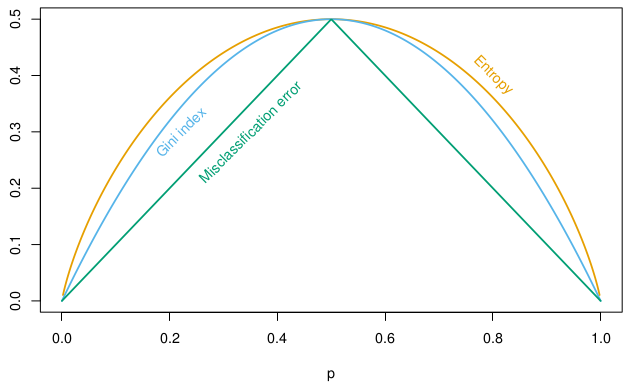
\includegraphics[width=\textwidth]{figure9_3}
}


\frame{\frametitle{Classification trees: }
\framesubtitle{example}
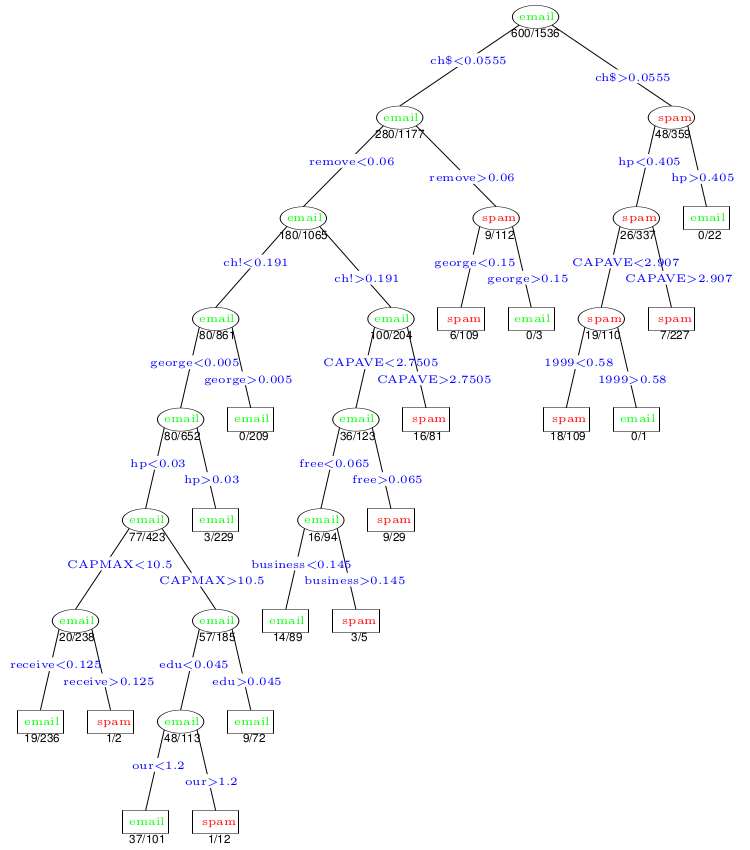
\includegraphics[width=\textwidth]{figure9_5}
}


\frame{\frametitle{Tree-based Methods: }
\framesubtitle{remarks}
Tree-based methods:
\begin{itemize}
 \item \textcolor{uio}{fast} to construct, \textcolor{uio}{interpretable} models;
 \item can incorporate \textcolor{uio}{mixtures} of \textcolor{uio}{numeric} and \textcolor{uio}{categorical} inputs;
 \item \textcolor{uio}{immune to outliers}, resistant to \textcolor{uio}{irrelevant} inputs;
 \item \textcolor{uio}{lack of smoothness};
 \item difficulty in capturing \textcolor{uio}{additive structures};
 \item \textcolor{uio}{highly unstable} (high variance).
\end{itemize}
}



\section{Bagging}

\subsection{Bootstrap aggregation}

\frame{\frametitle{Bagging: }
\framesubtitle{\cite{Galton1907}}
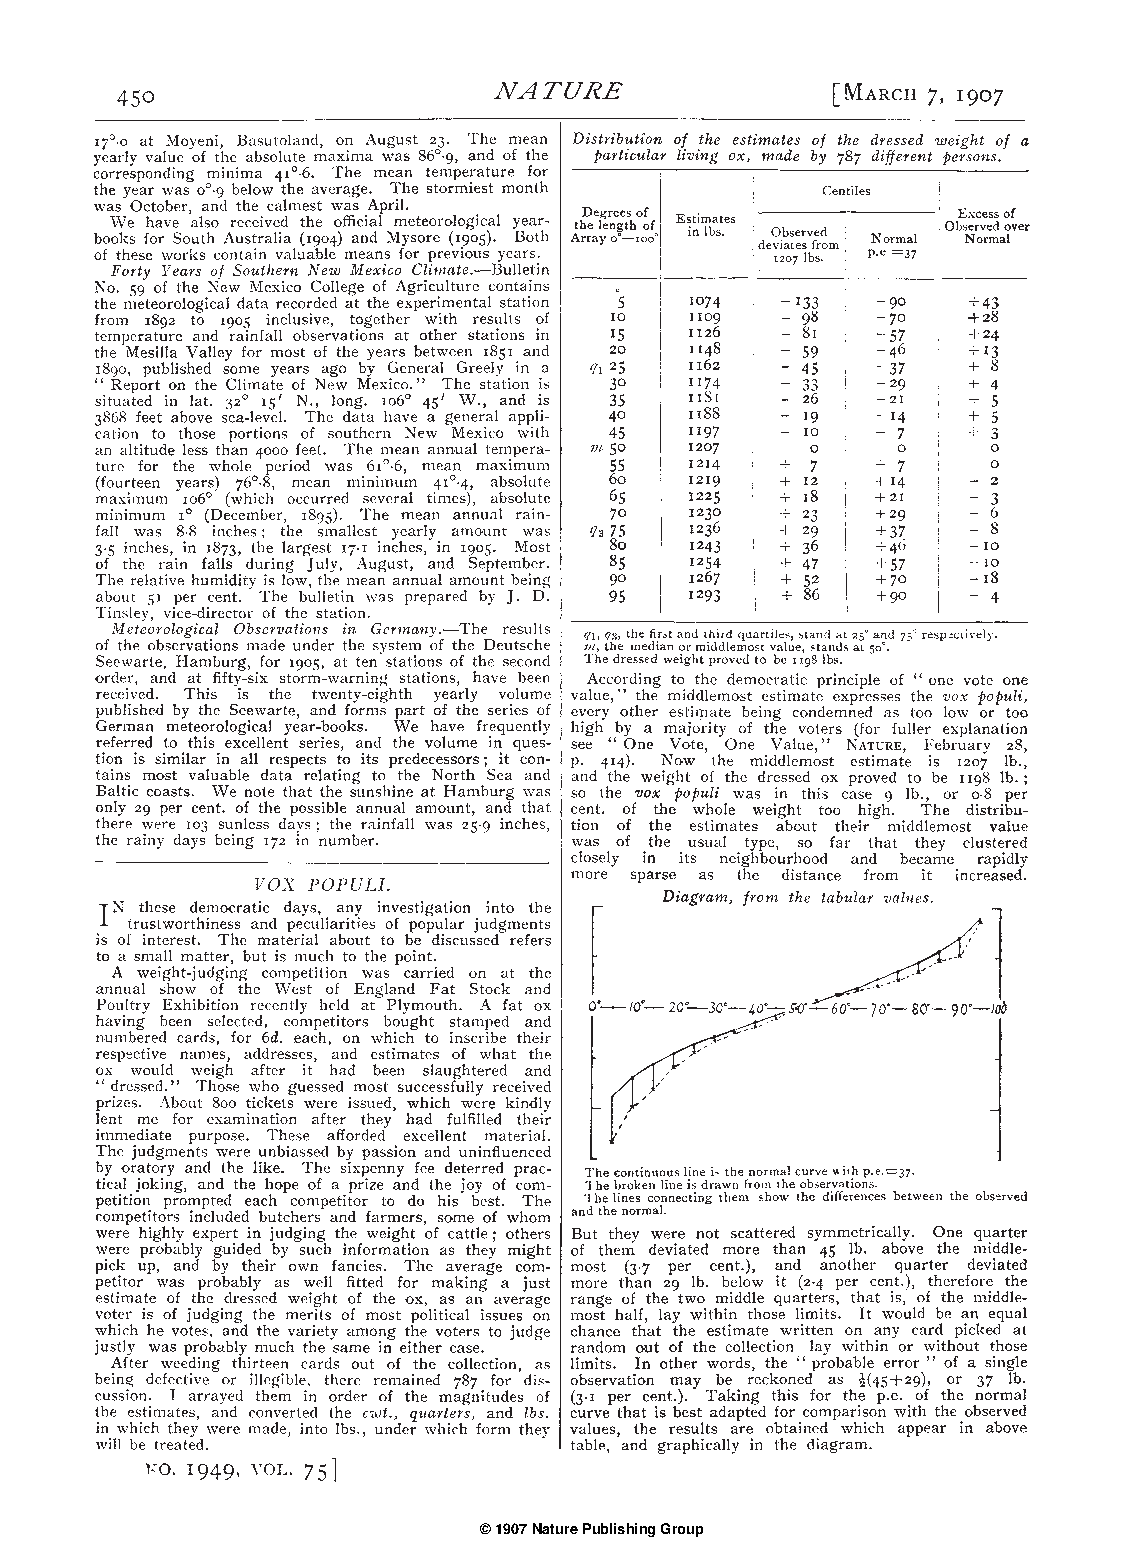
\includegraphics[width=\textwidth]{galton_1907}
}

\frame{\frametitle{Bagging: }
\framesubtitle{\cite{Galton1907}}
In 1907, Sir Francis Galton visited a country fair:

\vspace{12pt}

{\it A weight-judging competition was carried on at the annual show of the West of England Fat Stock and  Poultry Exhibition recently held at Plymouth. A fat ox having been selected, competitors bought stamped 
and numbered cards [\dots] on which to inscribe their respective names, addresses, and estimates of what the ox would weigh after it had been slaughtered and ``dressed''. Those who guessed most successfully received prizes. About 800 tickets were issued, which were kindly lent me for examination after they  had fulfilled their immediate purpose.} 
}

\frame{\frametitle{Bagging: }
\framesubtitle{\cite{Galton1907}}
After having arrayed and analyzed the data, \cite{Galton1907} stated:

\vspace{12pt}

{\it It appears then, in this particular instance, that the \textcolor{uio}{vox populi is correct to within 1 per cent} of the real value, and that the individual estimates are abnormally distributed in such a way that it is an equal chance whether one of them, selected at random, \textcolor{uio}{falls within or without the limits of -3.7 per cent and +2.4 per cent} of their middlemost value.} 

\vspace{12pt}

Concept of ``{\bf \uline{Wisdom of Crowds}}'' \citep[or, as][``how it is that a committee of blockheads can somehow arrive at a highly reasoned decision, despite the weak judgement of the individual members.'']{ShapireFreund2014}
}

\frame{\frametitle{Bagging: }
\framesubtitle{wisdom of crowds}
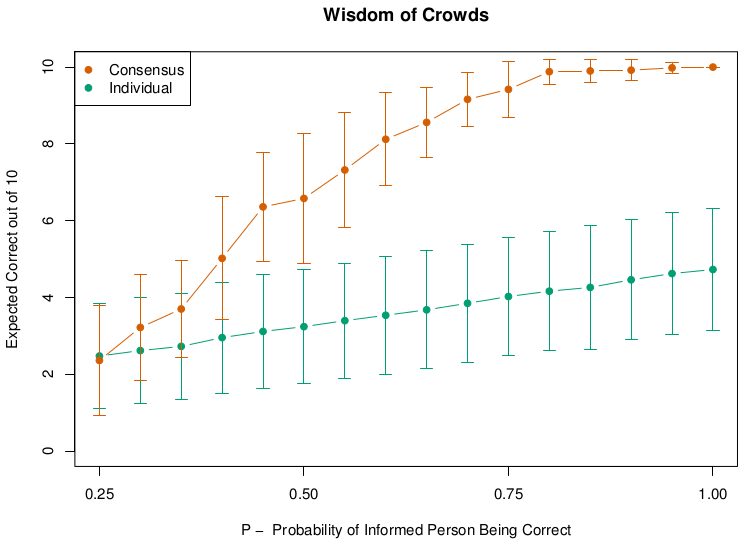
\includegraphics[width=0.98\textwidth]{figure8_11}
}


\subsection{Bootstrap trees}

\frame{\frametitle{Bagging: }
\framesubtitle{translate this message into trees}
How do can we \textcolor{uio}{translate} this idea into \textcolor{uio}{tree-based methods}?
\begin{itemize}
\item we can \textcolor{uio}{fit several trees}, then \textcolor{uio}{aggregate} their results;
\item problems:
\begin{itemize}
 \item ``individuals'' are supposed to be \textcolor{uio}{independent};
 \item we have \textcolor{uio}{only one} dataset \dots
 \end{itemize} 
 \item[]
\end{itemize}
How can we mimic different datasets while having only one?
}


\frame{\frametitle{Bagging: }
\framesubtitle{the solution is \dots}
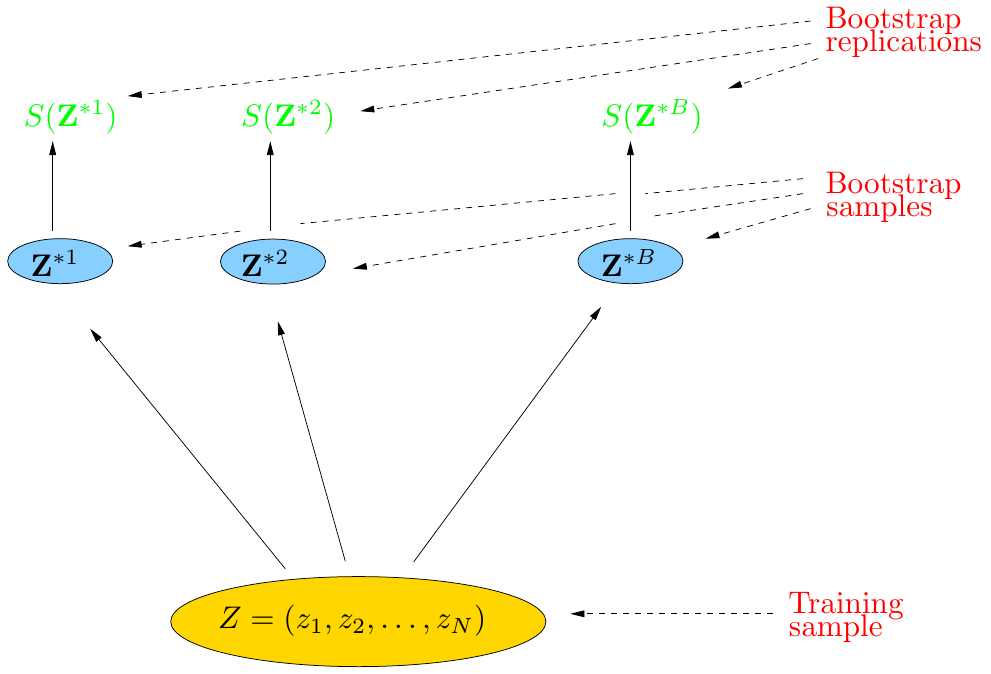
\includegraphics[width=\textwidth]{fig7_12}
}


\frame{\frametitle{Bagging: }
\framesubtitle{bootstrap trees}
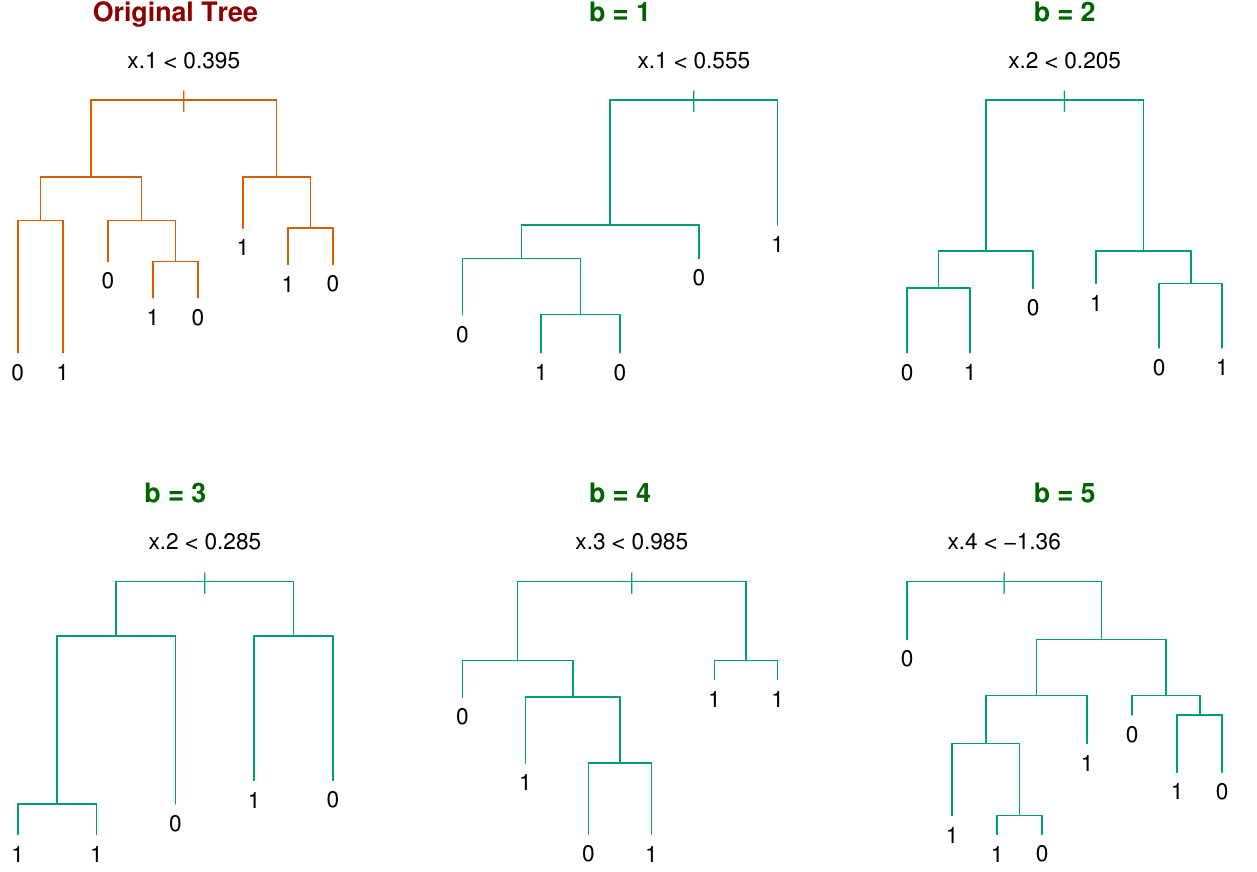
\includegraphics[width=\textwidth]{fig8_9}
}


\frame{\frametitle{Bagging: }
\framesubtitle{bootstrap trees}
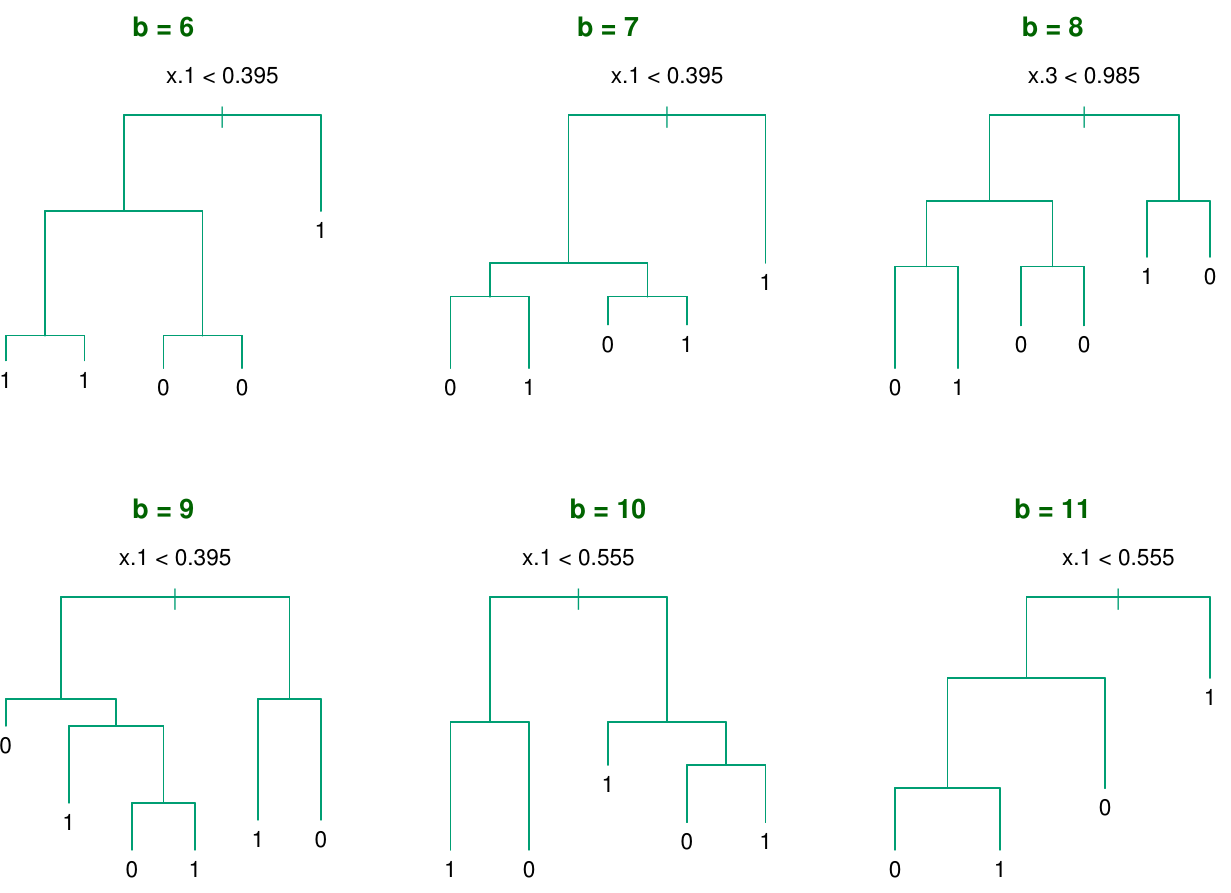
\includegraphics[width=0.98\textwidth]{fig8_92}
}


\frame{\frametitle{Bagging: }
\framesubtitle{bootstrap trees}
The procedure so far:
\begin{itemize}
\item generate \textcolor{uio}{bootstrap samples};
\item \textcolor{uio}{fit} a tree on each bootstrap sample;
\item obtain \textcolor{uio}{$B$ trees}.
\end{itemize}

\vspace{12pt}

At this point, \textcolor{uio}{aggregate the results}. How?
\begin{itemize}
\item {\bf consensus}: $\hat{G}(x) = \text{argmax}_k \, q_k(x)$, $k \in \{1, \dots, K\}$,
\begin{itemize}
\item where $q_k(x)$ is the \textcolor{uio}{proportion of trees} voting for the category $k$;
\end{itemize}
\item {\bf probability}: $\hat{G}(x) = \text{argmax}_k \, B^{-1}\sum_{b=1}^B p_k^{[b]}(x)$, $k \in \{1, \dots, K\}$,
\begin{itemize}
\item where $p_k^{[b]}(x)$ is the \textcolor{uio}{probability assigned} by the $b$-th tree to category $k$;
\end{itemize}
\end{itemize}
}


\frame{\frametitle{Bagging: }
\framesubtitle{bootstrap trees}
\centering
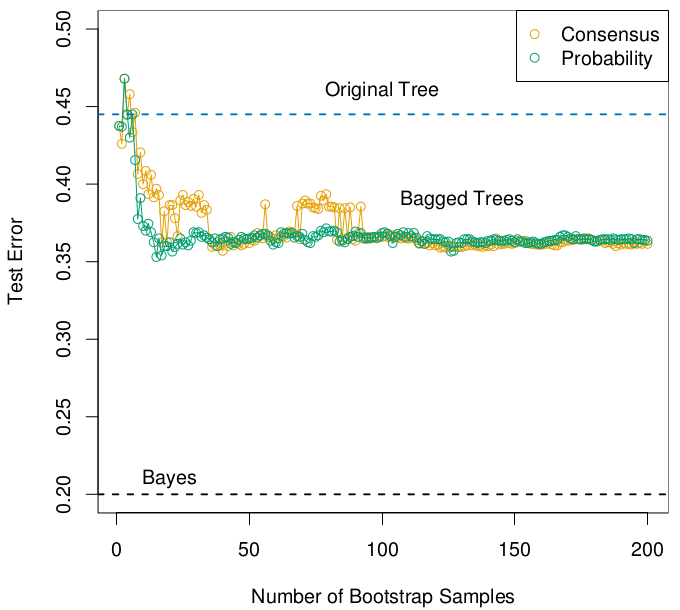
\includegraphics[width=0.78\textwidth]{figure8_10}
}


\frame{\frametitle{Bagging: }
\framesubtitle{general}
In general, consider the \textcolor{uio}{training data} $Z = \{(y_1,x_1), \dots, (y_N,x_N)\}$.
The {\bf \uline{bagging}} ({\bf b}oostrap {\bf agg}regat{\bf ing}) estimate is define by
$$
\hat{f}_\text{bag}(x) = E_{\hat{\mathcal{P}}}[\hat{f}^*(x)],
$$
where:
\begin{itemize}
\item $\hat{\mathcal{P}}$ is the \textcolor{uio}{empirical distribution} of the data $(y_i, x_i)$;
\item $\hat{f}^*(x)$ is the \textcolor{uio}{prediction} computed on a bootstrap sample $Z^*$;
\item i.e., $(y^*_i, x^*_i) \sim \hat{\mathcal{P}}$.
\end{itemize}

\vspace{6pt}

The \textcolor{uio}{empirical version} of the bagging estimate is
$$
\hat{f}_\text{bag}(x) = \frac{1}{B} \sum_{b=1}^B \hat{f}^*(x),
$$
where $B$ is the number of bootstrap samples.
}


\frame{\frametitle{Bagging: }
\framesubtitle{variance}
Bagging has \textcolor{uio}{smaller prediction error} because it \textcolor{uio}{reduces the variance} component,
\begin{align*}
E_\mathcal{P}[(Y - \hat{f}^*(x))^2] &= E_\mathcal{P}[(Y - f_\text{bag}(x) + f_\text{bag}(x) - \hat{f}^*(x))^2]\\
  &= E_\mathcal{P}[(Y - f_\text{bag}(x))^2] + E_\mathcal{P}[(f_\text{bag}(x) - \hat{f}^*(x))^2]\\
  &\geq E_\mathcal{P}[(Y - f_\text{bag}(x))^2],
\end{align*}
where $\mathcal{P}$ is the data distribution.

\vspace{12pt}

Note that this \textcolor{uio}{does not work} for \textcolor{uio}{0-1 loss}:
\begin{itemize}
\item due to \textcolor{uio}{non-additivity} of bias and variance;
\item bagging makes \textcolor{uio}{better} a \textcolor{uio}{good} classifier, \textcolor{uio}{worse} a \textcolor{uio}{bad} one.
\end{itemize}
}


\frame{\frametitle{Bagging: }
\framesubtitle{from bagging to random forests}
The average of $B$ identically distributed r.v.\ with variance $\sigma^2$ and \textcolor{uio}{positive pairwise correlation} $\rho$ has variance
$$
\rho\sigma^2 + \frac{1-\rho}{B} \sigma^2.
$$
\begin{itemize}
\item as $B$ increases, the \textcolor{uio}{second term goes to 0};
\item the \textcolor{uio}{bootstrap trees} are p.\ \textcolor{uio}{correlated} $\rightarrow$ first term dominates.
\item[] \centering $\downarrow$
\item[] construct bootstrap tree \textcolor{uio}{as less correlated as possible}
\item[] $\downarrow$
\item[] {\bf \uline{random forests}}
\end{itemize}
}


\frame{\frametitle{Bagging: }
\framesubtitle{from bagging to boosting}
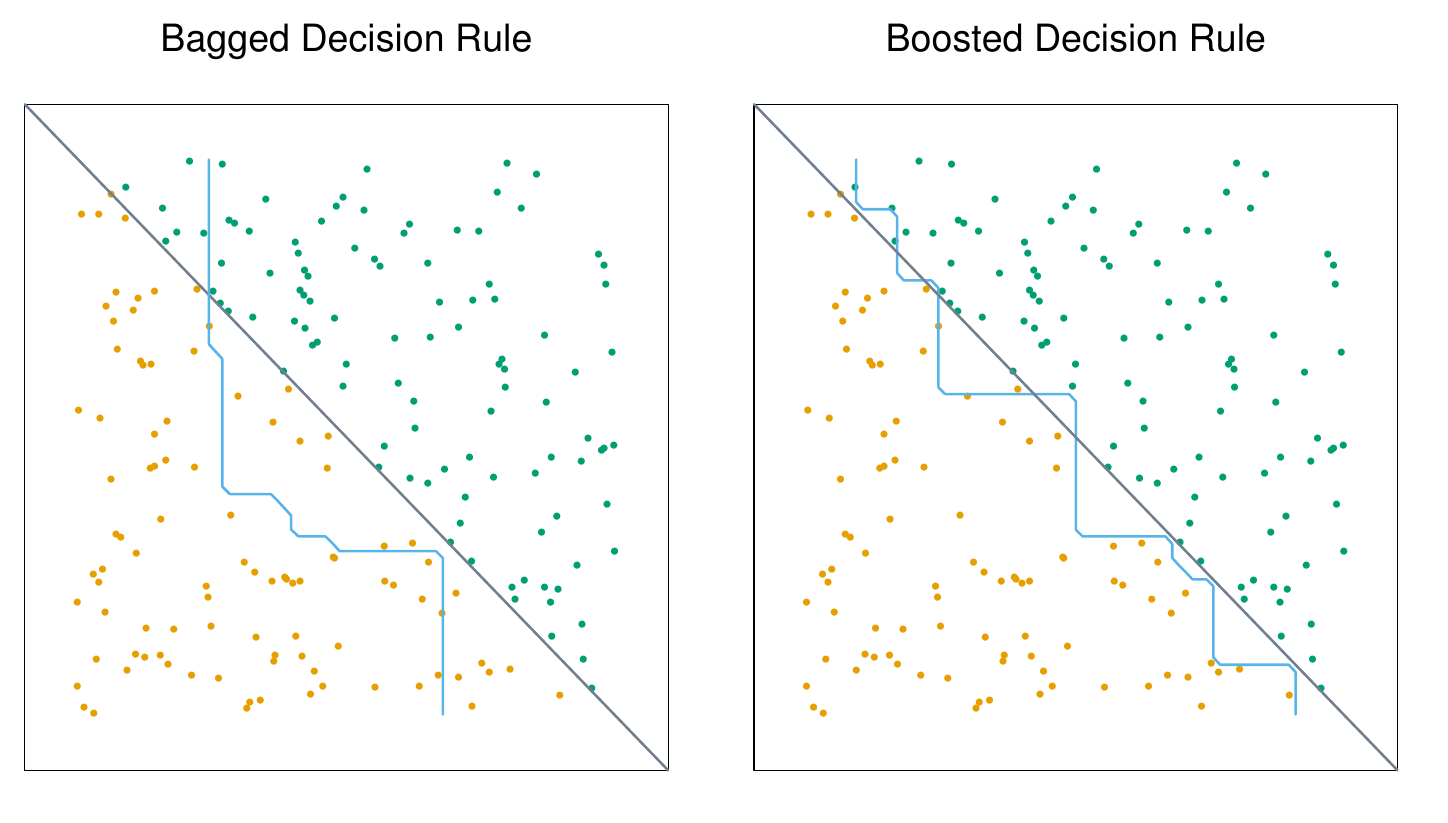
\includegraphics[width=\textwidth]{fig8_12}
}




%%%%%%%%%%%
\section*{Bibliography}
%%%%%%%%%%%

\frame[allowframebreaks]{\frametitle{References}
\footnotesize
\bibliographystyle{../../../../support/biometrika}
\bibliography{../../../../support/biblio}
}

\end{document}
